\documentclass[a4paper]{article}
\usepackage{graphicx}
\usepackage{amsmath, amsfonts, geometry, float, listings, enumerate, multicol}
\usepackage{multicol, float, color, colortbl}
\usepackage{tikz, titlesec, parskip, pgfplots, filecontents}
\usepackage{hyperref}
\usepackage{amsmath}
\usepackage{tikz, titlesec, parskip}
\usepackage{tikz,pgfplots}
\usepackage[americanvoltages,fulldiodes,siunitx]{circuitikz}
\usetikzlibrary{shapes,arrows}
\usepackage{enumitem}
\usepackage{circuitikz}

\titlespacing{\section}{0pt}{10pt}{0pt}
\titlespacing{\subsection}{0pt}{10pt}{0pt}
\titlespacing{\subsubsection}{0pt}{10pt}{0pt}

\usetikzlibrary{calc,patterns,through}
\newcommand{\arcangle}{%
	\mathord{<\mspace{-9mu}\mathrel{)}\mspace{2mu}}%
}

\renewcommand{\baselinestretch}{1.4}
 \geometry{
 a4paper,
 total={170mm,257mm},
 left=20mm,
 top=20mm,
 }
\usepackage{fancyhdr}
\usepackage{indentfirst}
\pagestyle{fancy}
\fancyhf{}
\rhead{\textbf{سیستم‌های مخابراتی}}
\lhead{\textbf{تمرین سری دوم}}
\cfoot{(\space \space \space \space \textbf{\thepage}  \space \space \space)}
\renewcommand{\headrulewidth}{1pt}
\renewcommand{\footrulewidth}{1pt}

 
\usepackage{xepersian}
\setlatintextfont{Times New Roman}
\settextfont{XB Niloofar}
\setdigitfont{XB Niloofar}
\DefaultMathsDigits

\makeatletter
\bidi@patchcmd{\@Abjad}{آ}{الف}
{\typeout{Succeeded in changing آ into الف}}
{\typeout{Failed in changing آ into الف}}
\makeatother
\PersianAlphs

\begin{document}
\begin{minipage}{0.6\textwidth}
\begin{bf}
\begin{center}
	به نام خدا\\
	\vspace{0.25cm}
	دانشگاه صنعتی شریف\\
	\vspace{0.25cm}
	دانشکده مهندسی برق\\
	\vspace{0.5cm}

\large
گروه دکتر پاکروان - سیستم‌های مخابراتی \\
نیم سال اول
۱۴۰۱-۱۴۰۰\\
\Large
\vspace{0.4cm}
تمرین عملی سری دوم\\
\end{center}
\end{bf}
\normalsize
\end{minipage} \hfill
\begin{minipage}{0.35\textwidth}
\begin{flushleft}
\includegraphics[width=0.6\textwidth]{Shariflogo.png}\\ \large
\end{flushleft}

 \end{minipage}
\\

\rule[0.1\baselineskip]{\textwidth}{1.5pt}

\large

\section*{
لطفاً به نکات زیر توجه بفرمایید:
}
\begin{enumerate}
	\item 
نتایج و پاسخ های خود را در یک فایل با فرمت zip به نام
\LR{HW$2$-Name-StudentNumber}
 در سایت  cw قرار دهید.
	\item 
کسب نمره کامل در هر سؤال مستلزم تحویل  \textbf{کدها} و \textbf{توضیحات} می‌باشد. 
\item 
برای سؤالات، باید روشی که استفاده کرده‌اید را توضیح  و نتایجی که گرفته‌اید را ارائه دهید. این توضیحات می‌تواند در یک فایل  pdf باشد.
\item 
کدهای خود را خوانا بنویسید و کامنت‌‌گذاری کنید.
\item
ابهام يا اشكالات خود را مي توانيد  از طریق
\href{https://t.me/Amirhosein_javadi}{@Amirhosein\_Javadi}
یا 
\href{mailto:javadiamirhosein.2000@gmail.com}{\LR{Javadiamirhosein.$2000$@gmail.com}}
مطرح نماييد.
\item 
کدهای شما تماماً باید توسط خودتان نوشته شده باشند. هرگونه استفاده از کد دیگران به هر شکل ممکن، تقلب محسوب می‌شود و نمره تمرین کامپیوتری جاری صفر خواهد شد. پس در هیچ صورت کدهای خود را برای دیگران ارسال نکنید.

\item 
مهلت تحویل:  
\end{enumerate}
\clearpage


\section{\lr{Envelope Detector}} 
در این سوال قصد داریم با شبیه‌سازی یک مدار فیزیکی، پیام یک سیگنال 
\lr{AM}
 را به دست بیاوریم.
\\
در صورتی که سیگنال 
$ x_{c} $
یک سیگنال مدوله‌شده باشد، با انتخاب مناسب مقادیر
$R$
 و
$C$
می‌توانیم پوش سیگنال،
$\hat{m}$،
 را از اختلاف ولتاژ در دو سر مقاومت به دست بیاریم و سپس با حذف مقدار \lr{dc} پوش، پیام را بازیابی کنیم.
\begin{figure}[H]
\begin{center}
	\begin{circuitikz}
	\draw
	(5,0) to[C=$C$, ultra thin] (5,3)
	(6.5,0) to[R=$R$, ultra thin] (6.5,3)
	(3,3) to[empty diode, ultra thin] (4,3) 
	(1.5,3) to [open, v=$x_{c}$] (1.5,0)
	(6.8,3) to [open, v^>=$\hat{m}$] (6.8,0)
	(1.5,3) -- (3,3)
	(4,3) -- (6.5,3)
	(1.5,0) -- (6.5,0)
	;
	\end{circuitikz}
\end{center}
		\caption{\LR{Envelope Detector}}
	\label{Envelope Detector}
\end{figure}
پیام ارسالی را $ m(t) $ می‌نامیم:
\begin{equation*}
 	m(t) = \cos(5 \pi t)+\sin(8 \pi t) \qquad (0 \leq t \leq 1)
\end{equation*}
\begin{enumerate}
	\item 
این پیام را 
$ f_{s} = 10000 $
نمونه‌ برداری کنید.
سپس پیام را نرمالیزه کنید و با مقادیر زیر سیگنال 
$ x_{c} $
 را بسازید.
 \begin{equation*}
	x_{c}(t) = A_{c} (1+\mu m(t)) \cos(2 \pi f_{c} t) \qquad ( A_{c}=1, \mu =1, f_{c}=1000)
\end{equation*}
	\item 
پیام
$ m(t) $
 را به وسیله‌ی 
\lr{Envelope Detector}
از سیگنال 
$ x_{c}(t) $
با مقدار‌های مناسب برای مقاومت و خازن به دست بیاورید. 
\item 
 در یک نمودار، پیام، سیگنال \lr{AM} ارسالی، پوش سیگنال \lr{AM} به دست آمده و پیام استخراج‌شده‌ را رسم کنید.
\end{enumerate}

\section{\lr{USSB Modulation}} 
\begin{enumerate}
	\item
سه پیام زیر را با نرخ نمونه‌برداری 
$ f_{s} = 10000 $
برای لحظات 
$ 0 \leq t \leq 9 $
 نمونه‌برداری کنید.
\begin{gather*}
	x_1(t) = (\cos(10 \pi t)+ \sin(12 \pi t)) (u(t)-u(t-3)) \quad \qquad (f_{c1} = 500)
	\\
	x_2(t) = (\cos(14 \pi t)+ \sin(8 \pi t)) (u(t-3)-u(t-6)) \qquad (f_{c2} = 650)
	\\
	x_3(t) = (\cos(5 \pi t)+ \sin(15 \pi t)) (u(t-6)-u(t-9)) \qquad (f_{c3} = 800)
\end{gather*}
\item
این سه پیام را با فرکانس‌ مرکزی مربوط به هر پیام که روبه‌روی آن نوشته‌شده‌ بود به صورت
 \lr{USSB} 
مدوله کنید و این سه سیگنال مدوله‌شده را با هم جمع کنید و به سیگنال ارسالی برسید. می‌توانید از دستور
\lr{\texttt{ssbmod}}
استفاده کنید و یا با استفاده از تبدیل هیلبرت مدولاسیون 
\lr{ssb}
را پیاده‌سازی کنید.
\item
در یک نمودار، سه‌ پیام، سه سیگنال مدوله‌شده و سیگنال ارسالی را رسم کنید.
\item
 در یک نمودار، اندازه‌ی فوریه‌ی سیگنال‌‌های قسمت قبل را رسم کنید.
\item
سیگنال ارسالی را از یک کانال نویزی با
 $ Snr = 5db $
 بگذرانید. برای کاهش اثر نویز، از یک فیلتر \lr{bandpass} استفاده کنید تا نویز‌هایی با فرکانس خارج باند فرکانس سیگنال ارسالی حذف شوند.
 در یک نمودار، اندازه‌ی فوریه‌ی سیگنال دریافتی و اندازه‌ی فوریه‌ی سیگنال خروجی فیلتر \lr{bandpass} را رسم کنید.
\item
  سه پیام ارسالی را از سیگنال خروجی فیلتر \lr{bandpass} استخراج کنید. در یک نمودار، سه پیام ارسالی و سه پیام دریافت شده را رسم کنید. می‌توانید از دستور
  \lr{\texttt{ssbdemod}}
  استفاده کنید.
\end{enumerate}
\section{\lr{FM Modulation}}
در این بخش می‌خواهیم با سه روش پیام ارسالی را از سیگنال مدوله‌شده‌ی  
\lr{FM}
اش به دست بیاوریم.
 
پیام ارسالی را $ m(t) $ می‌نامیم و داریم:
\begin{equation*}
	m(t) = \sin(25 \pi t) \qquad (0 \leq t \leq 1)
\end{equation*}
\begin{enumerate}
	\item 
این پیام را 
$ f_{s} = 10000 $
نمونه‌ برداری کنید و با مقادیر زیر سیگنال \lr{FM} را به کمک دستور
 \lr{\texttt{fmmod}}
  به دست بیاورید.
 \begin{equation*}
	x_{c}(t) = A_{c} \cos(2 \pi f_c t + 2 \pi f_{\triangle} \int_{0}^{t} m(\tau) d\tau) \qquad (A_{c}=1, \; Fc = 200, \; f_{\triangle}=30)
\end{equation*}
	\item 
	با کمک دستور
	  \lr{\texttt{fmdemod}}
	  سیگنال پیام را به صورت ایده‌آل بازیابی کنید.
	\item 
	با مشتق گرفتن از سیگنال 
	$ x_{c} $
	خواهیم داشت:
	 \begin{equation*}
	x_{d}(t) = \frac{dx_{c}(t)}{dt} = -A_{c} (2 \pi f_c + 2 \pi f_{\triangle} m(t))\sin(2 \pi f_c t + 2 \pi f_{\triangle} \int_{0}^{t} m(\tau) d\tau) 
	\end{equation*}
در صورتی که تغییرات فرکانس سیگنال 
	$ \sin(2 \pi f_c t + 2 \pi f_{\triangle} \int_{0}^{t} m(\tau) d\tau) $
	به دلیل پیام
	$ m(t) $
	نسبت به فرکانس
	$ f_c $
	قایل صرف نظر باشد یعنی
	$ \frac{f_{\triangle} m(t)}{ f_c} \approx 0 $،
	 می‌توانیم سیگنال 
	$ x_{d} $
را یک سیگنال
\lr{AM}
در نظر بگیریم که پوش آن حاوی پیام مورد نظر است.
با کمک 
\lr{Envelope Detector}
ساخته‌شده در سوال اول با مقدار‌های جدید برای مقاومت و خازن پیام را بازیابی کنید.
	\item 
راه دیگری آشکار‌سازی پیام 
\lr{Zero Crossing Detector}
است. از آن‌ جایی که مقدار پیام در فرکانس لحظه‌ای سیگنال \lr{FM}تاثیرگذار است، انتظار داریم زمانی که مقدار پیام در ماکزیمم است فرکانس لحظه‌ای زیاد باشد و بالعکس. فرکانس سیگنال را با تعداد عبور از صفر می‌توان تخمین زد. در واقع، زمانی که فرکانس زیاد است انتظار داریم سیگنال با نرخ قابل توجهی از صفر عبور پیدا کند و بالعکس. پس برای آشکار سازی پیام از سیگنال \lr{FM}، می‌توانیم از بلوک دیاگرامی مانند بلوک دیاگرام شکل \ref{ZCD} استفاده ‌کنیم :
\begin{figure}[H]
	\begin{center}
		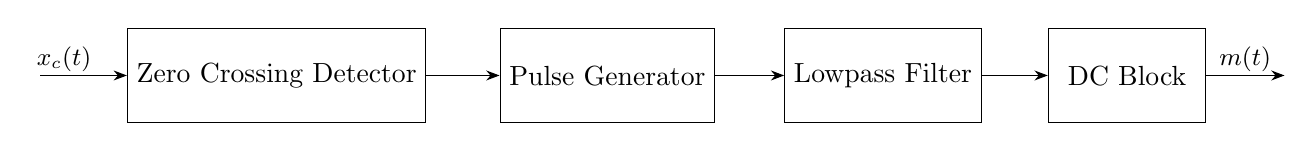
\begin{tikzpicture}
			[
			block/.style={draw, minimum width=20mm, minimum height=12mm},
			sum/.style={circle, draw, minimum size=6mm, inner sep=0pt,
				node contents={\huge$+$}},
			mult/.style={circle, draw, minimum size=6mm, inner sep=0pt},
			>=Stealth,
			node distance=12mm and 10mm]
			\coordinate (in) at (-1.7,0) [];
			\node (ZCD) [block]  at (1.3,0) {\lr{Zero Crossing Detector}};
			\node (PG) [block]  at (5.5,0) {\lr{Pulse Generator}};
			\node (LPF) [block]  at (8.3+0.7,0) {\lr{Lowpass Filter}};
			\node (DCB) [block]  at (11.4+0.7,0) {\lr{DC Block}};
			\coordinate (out) at (14.1,0) [];
			\draw[->]   (in) -- (ZCD);
			\draw[->]   (ZCD) -- (PG);
			\draw[->]   (PG) -- (LPF);
			\draw[->]   (LPF) -- (DCB);
			\draw[->]   (DCB) -- (out);			
			\draw (-1.4,0.2) node[centered]  {\small $ x_c(t) $};
			%\draw (-2,0.2) node[centered]  {\small Received  signal(t)};
			\draw (13.6,0.2) node[centered]{\small  $ m(t) $};
		\end{tikzpicture}
		\caption{\LR{Zero Crossing Detector}}
		\label{ZCD}
	\end{center}
\end{figure}
برای پیاده‌سازی بلوک 
\lr{Zero Crossing Detector}
می‌توانید از سیگنال
\lr{sign($x_c(t)$)}
مشتق بگیرید و سپس قدرمطلق سیگنال را به عنوان مکان‌هایی که از صفر گذر کردید در نظر بگیرید. خروجی این بلوک باید فقط در زمان‌هایی که عبور از صفر داشته‌ایم مقدار یک و در بقیه‌ زمان‌ها صفر باشد. بلوک 
\lr{Pulse Generator}
باید به ازای هر گذر از صفر یک پالس مستطیلی به مدت محدود تولید کند. با استفاده‌ از این روش پیام را بازیابی کنید.
\item
در یک نمودار، پیام، سیگنال \lr{FM} پیام و پیام‌های بازیابی شده در سه روش را رسم کنید.
\end{enumerate}
\end{document}
